% Options for packages loaded elsewhere
% Options for packages loaded elsewhere
\PassOptionsToPackage{unicode}{hyperref}
\PassOptionsToPackage{hyphens}{url}
\PassOptionsToPackage{dvipsnames,svgnames,x11names}{xcolor}
%
\documentclass[
  english,
  10pt,
  letterpaper,
  DIV=11,
  numbers=noendperiod]{scrartcl}
\usepackage{xcolor}
\usepackage[margin=1in]{geometry}
\usepackage{amsmath,amssymb}
\setcounter{secnumdepth}{5}
\usepackage{iftex}
\ifPDFTeX
  \usepackage[T1]{fontenc}
  \usepackage[utf8]{inputenc}
  \usepackage{textcomp} % provide euro and other symbols
\else % if luatex or xetex
  \usepackage{unicode-math} % this also loads fontspec
  \defaultfontfeatures{Scale=MatchLowercase}
  \defaultfontfeatures[\rmfamily]{Ligatures=TeX,Scale=1}
\fi
\usepackage{lmodern}
\ifPDFTeX\else
  % xetex/luatex font selection
\fi
% Use upquote if available, for straight quotes in verbatim environments
\IfFileExists{upquote.sty}{\usepackage{upquote}}{}
\IfFileExists{microtype.sty}{% use microtype if available
  \usepackage[]{microtype}
  \UseMicrotypeSet[protrusion]{basicmath} % disable protrusion for tt fonts
}{}
\makeatletter
\@ifundefined{KOMAClassName}{% if non-KOMA class
  \IfFileExists{parskip.sty}{%
    \usepackage{parskip}
  }{% else
    \setlength{\parindent}{0pt}
    \setlength{\parskip}{6pt plus 2pt minus 1pt}}
}{% if KOMA class
  \KOMAoptions{parskip=half}}
\makeatother
% Make \paragraph and \subparagraph free-standing
\makeatletter
\ifx\paragraph\undefined\else
  \let\oldparagraph\paragraph
  \renewcommand{\paragraph}{
    \@ifstar
      \xxxParagraphStar
      \xxxParagraphNoStar
  }
  \newcommand{\xxxParagraphStar}[1]{\oldparagraph*{#1}\mbox{}}
  \newcommand{\xxxParagraphNoStar}[1]{\oldparagraph{#1}\mbox{}}
\fi
\ifx\subparagraph\undefined\else
  \let\oldsubparagraph\subparagraph
  \renewcommand{\subparagraph}{
    \@ifstar
      \xxxSubParagraphStar
      \xxxSubParagraphNoStar
  }
  \newcommand{\xxxSubParagraphStar}[1]{\oldsubparagraph*{#1}\mbox{}}
  \newcommand{\xxxSubParagraphNoStar}[1]{\oldsubparagraph{#1}\mbox{}}
\fi
\makeatother


\usepackage{longtable,booktabs,array}
\newcounter{none} % for unnumbered tables
\usepackage{calc} % for calculating minipage widths
% Correct order of tables after \paragraph or \subparagraph
\usepackage{etoolbox}
\makeatletter
\patchcmd\longtable{\par}{\if@noskipsec\mbox{}\fi\par}{}{}
\makeatother
% Allow footnotes in longtable head/foot
\IfFileExists{footnotehyper.sty}{\usepackage{footnotehyper}}{\usepackage{footnote}}
\makesavenoteenv{longtable}
\usepackage{graphicx}
\makeatletter
\newsavebox\pandoc@box
\newcommand*\pandocbounded[1]{% scales image to fit in text height/width
  \sbox\pandoc@box{#1}%
  \Gscale@div\@tempa{\textheight}{\dimexpr\ht\pandoc@box+\dp\pandoc@box\relax}%
  \Gscale@div\@tempb{\linewidth}{\wd\pandoc@box}%
  \ifdim\@tempb\p@<\@tempa\p@\let\@tempa\@tempb\fi% select the smaller of both
  \ifdim\@tempa\p@<\p@\scalebox{\@tempa}{\usebox\pandoc@box}%
  \else\usebox{\pandoc@box}%
  \fi%
}
% Set default figure placement to htbp
\def\fps@figure{htbp}
\makeatother


% definitions for citeproc citations
\NewDocumentCommand\citeproctext{}{}
\NewDocumentCommand\citeproc{mm}{%
  \begingroup\def\citeproctext{#2}\cite{#1}\endgroup}
\makeatletter
 % allow citations to break across lines
 \let\@cite@ofmt\@firstofone
 % avoid brackets around text for \cite:
 \def\@biblabel#1{}
 \def\@cite#1#2{{#1\if@tempswa , #2\fi}}
\makeatother
\newlength{\cslhangindent}
\setlength{\cslhangindent}{1.5em}
\newlength{\csllabelwidth}
\setlength{\csllabelwidth}{3em}
\newenvironment{CSLReferences}[2] % #1 hanging-indent, #2 entry-spacing
 {\begin{list}{}{%
  \setlength{\itemindent}{0pt}
  \setlength{\leftmargin}{0pt}
  \setlength{\parsep}{0pt}
  % turn on hanging indent if param 1 is 1
  \ifodd #1
   \setlength{\leftmargin}{\cslhangindent}
   \setlength{\itemindent}{-1\cslhangindent}
  \fi
  % set entry spacing
  \setlength{\itemsep}{#2\baselineskip}}}
 {\end{list}}
\usepackage{calc}
\newcommand{\CSLBlock}[1]{\hfill\break\parbox[t]{\linewidth}{\strut\ignorespaces#1\strut}}
\newcommand{\CSLLeftMargin}[1]{\parbox[t]{\csllabelwidth}{\strut#1\strut}}
\newcommand{\CSLRightInline}[1]{\parbox[t]{\linewidth - \csllabelwidth}{\strut#1\strut}}
\newcommand{\CSLIndent}[1]{\hspace{\cslhangindent}#1}

\ifLuaTeX
\usepackage[bidi=basic,shorthands=off]{babel}
\else
\usepackage[bidi=default,shorthands=off]{babel}
\fi
\ifLuaTeX
  \usepackage{selnolig} % disable illegal ligatures
\fi


\setlength{\emergencystretch}{3em} % prevent overfull lines

\providecommand{\tightlist}{%
  \setlength{\itemsep}{0pt}\setlength{\parskip}{0pt}}



 


\KOMAoption{captions}{tableheading}
\makeatletter
\@ifpackageloaded{caption}{}{\usepackage{caption}}
\AtBeginDocument{%
\ifdefined\contentsname
  \renewcommand*\contentsname{Table of contents}
\else
  \newcommand\contentsname{Table of contents}
\fi
\ifdefined\listfigurename
  \renewcommand*\listfigurename{List of Figures}
\else
  \newcommand\listfigurename{List of Figures}
\fi
\ifdefined\listtablename
  \renewcommand*\listtablename{List of Tables}
\else
  \newcommand\listtablename{List of Tables}
\fi
\ifdefined\figurename
  \renewcommand*\figurename{Figure}
\else
  \newcommand\figurename{Figure}
\fi
\ifdefined\tablename
  \renewcommand*\tablename{Table}
\else
  \newcommand\tablename{Table}
\fi
}
\@ifpackageloaded{float}{}{\usepackage{float}}
\floatstyle{ruled}
\@ifundefined{c@chapter}{\newfloat{codelisting}{h}{lop}}{\newfloat{codelisting}{h}{lop}[chapter]}
\floatname{codelisting}{Listing}
\newcommand*\listoflistings{\listof{codelisting}{List of Listings}}
\makeatother
\makeatletter
\makeatother
\makeatletter
\@ifpackageloaded{caption}{}{\usepackage{caption}}
\@ifpackageloaded{subcaption}{}{\usepackage{subcaption}}
\makeatother
\usepackage{bookmark}
\IfFileExists{xurl.sty}{\usepackage{xurl}}{} % add URL line breaks if available
\urlstyle{same}
% fallback for those not using the hyperref driver hyperxmp:
\makeatletter
\@ifundefined{xmpquote}{\newcommand{\xmpquote}[1]{#1}}{}
\makeatother
\hypersetup{
  pdftitle={Fourier Pricing of Spread and Basket Options under Stochastic Correlation},
  pdfauthor={Complex--Itô Random-Walk Research Project},
  pdflang={en},
  pdfkeywords={\xmpquote{spread options}, \xmpquote{basket
options}, \xmpquote{stochastic correlation}, \xmpquote{COS
method}, \xmpquote{characteristic function}, \xmpquote{implied
correlation}},
  colorlinks=true,
  linkcolor={blue},
  filecolor={Maroon},
  citecolor={Blue},
  urlcolor={Blue},
  pdfcreator={LaTeX via pandoc}}


\title{Fourier Pricing of Spread and Basket Options under Stochastic
Correlation}
\usepackage{etoolbox}
\makeatletter
\providecommand{\subtitle}[1]{% add subtitle to \maketitle
  \apptocmd{\@title}{\par {\large #1 \par}}{}{}
}
\makeatother
\subtitle{One-Dimensional Characteristic Functions from Real-Potential
Resolvents, COS Inversion, and Opposite-Curvature Implied-Correlation
Smiles}
\author{Complex--Itô Random-Walk Research Project}
\date{August 21, 2026}
\begin{document}
\maketitle
\begin{abstract}
Under a stochastic-correlation model in which two Brownian assets are
correlated through a bounded factor \(\rho_t=X_t/\sqrt{X_t^2+c^2}\) with
independent Gaussian driver, any linear combination
\(Z=\alpha_1F_1+\alpha_2F_2\) is conditionally Gaussian given the
correlation path, with Dambis--Dubins--Schwarz clock
\(v=\beta T+\alpha A_T\), \(A_T=\int_0^T\rho_sds\). We prove that the
discounted characteristic function of \(Z_T\) is exactly
one-dimensional, \[\phi_Z(u)=e^{-rT}e^{iuz_0-u^2\beta T/2}\,
L_A(\alpha u^2/2),\qquad L_A(s)=E[e^{-sA_T}],\] where \(L_A\) is a
real-potential Feynman--Kac resolvent. Boundedness of the factor
confines \(A_T\) to \((-T,T)\), so \(L_A\) exists for every real
argument --- the transform is globally defined. European prices follow
by Fang--Oosterlee cosine inversion or by quadrature against the exact
clock density; both deterministic routes agree to \(10^{-5}\) and match
Monte Carlo within four standard errors across strikes. Semi-analytic
Greeks follow as integrals against the clock density. Inverting
constant- correlation Bachelier quotes produces implied-correlation
smiles that are exactly symmetric in moneyness with opposite curvature
for spreads (wings down) and baskets (wings up), and ATM implied
correlation equal to \(E[A_T]\) --- falsifiable signatures absent from
the audited literature, where multi-asset Fourier methods require joint
characteristic functions and stochastic-correlation models are priced by
simulation.
\end{abstract}

\renewcommand*\contentsname{Table of contents}
{
\setcounter{tocdepth}{2}
\tableofcontents
}

\textbf{Mathematics Subject Classification (2020):} 91G20, 91G60, 65C05,
60H10.

\textbf{JEL classification:} G12, G13, C63.

\section{Introduction}\label{sec-introduction}

Spread and basket options are the canonical multi-asset derivatives, and
their pricing under \emph{stochastic} correlation is an unsolved
convenience: the audited multi-asset Fourier machinery ---
two-dimensional cosine expansions (Ruijter and Oosterlee 2012),
tensor-train decompositions ({Galetzka et al.} 2026), canonical-polyadic
compression --- all presuppose a known \textbf{joint} characteristic
function of the asset prices, and no stochastic-correlation model in the
audited corpus supplies one; practitioners fall back on Monte Carlo or
lower-bound approximations. Stochastic-correlation models themselves
(Teng et al. 2016) price quantos by conditional simulation around
Black--Scholes.

This paper closes the gap for the bounded-factor model. The key identity
is that conditional Gaussianity plus DDS reduce \(Z_T\) to a Gaussian
mixture whose mixing variable --- the occupation integral
\(A_T=\int_0^T\rho_sds\) --- has bounded support. The Laplace transform
\(L_A(s)=E[e^{-sA_T}]\) therefore exists for every real \(s\), is
computed by a single Feynman--Kac solve per mode with a \emph{real}
(non-oscillatory) potential, and assembles into an exact one-dimensional
characteristic function for \(Z_T\). Everything European about spreads
and baskets becomes deterministic.

Contributions:

\begin{enumerate}
\def\labelenumi{\arabic{enumi}.}
\tightlist
\item
  the exact global transform \(\phi_Z\) (Section~\ref{sec-cf});
\item
  two cross-validated deterministic pricers: resolvent+COS and
  clock-density quadrature (Section~\ref{sec-pricing});
\item
  semi-analytic delta/gamma/vegas (Section~\ref{sec-greeks});
\item
  the implied-correlation smile geometry: symmetric smiles, opposite
  curvature, ATM level \(=E[A_T]\) (Section~\ref{sec-smiles}).
\end{enumerate}

\section{Model and the exact transform}\label{sec-cf}

\subsection{Setup}\label{setup}

\[
dF_1=\sigma_1\,dW_1,\qquad
dF_2=\sigma_2(\rho_t\,dW_1+\sqrt{1-\rho_t^2}\,dW_2),
\]

\(\rho_t=f(X_t)=X_t/\sqrt{X_t^2+c^2}\), \(dX=\mu\,dt+\sigma\,dW\), with
the correlation driver independent of \((W_1,W_2)\). For weights
\((\alpha_1,\alpha_2)\) define

\[
Z=\alpha_1F_1+\alpha_2F_2,\qquad
\beta=\alpha_1^2\sigma_1^2+\alpha_2^2\sigma_2^2,\qquad
\alpha=2\alpha_1\alpha_2\sigma_1\sigma_2 .
\]

\subsection{Theorem (exact one-dimensional characteristic
function)}\label{theorem-exact-one-dimensional-characteristic-function}

\emph{Conditional on the correlation path,} \(Z_T\mid\rho\sim N(z_0,v)\)
\emph{with} \(v=\beta T+\alpha A_T\). \emph{Consequently}

\[
\phi_Z(u):=E\big[e^{-rT}e^{iuZ_T}\big]
=e^{-rT}e^{iuz_0-\frac12u^2\beta T}\;L_A\!\Big(\frac{\alpha u^2}{2}\Big),
\qquad L_A(s)=E\big[e^{-sA_T}\big],
\]

\emph{and \(L_A\) is given by the forward Feynman--Kac resolvent of the
driver with potential \(-sf(x)\).}

Because \(|A_T|<T\), \(0<L_A(s)\le e^{|s|T}\) for all real \(s\): no
moment explosion bounds the inversion strip, in contrast with
unbounded-variance models. The real potential makes each evaluation
numerically gentler than an oscillatory solve. Cross-validation: at
three frequencies the resolvent route and the clock-density route
(integrating \(e^{-u^2\alpha a/2}\) against the truncated-Fourier
density of \(A_T\)) agree to \(10^{-5}\) (Figure~\ref{fig-mgf}).

\begin{figure}[tbp]

\centering{

\pandocbounded{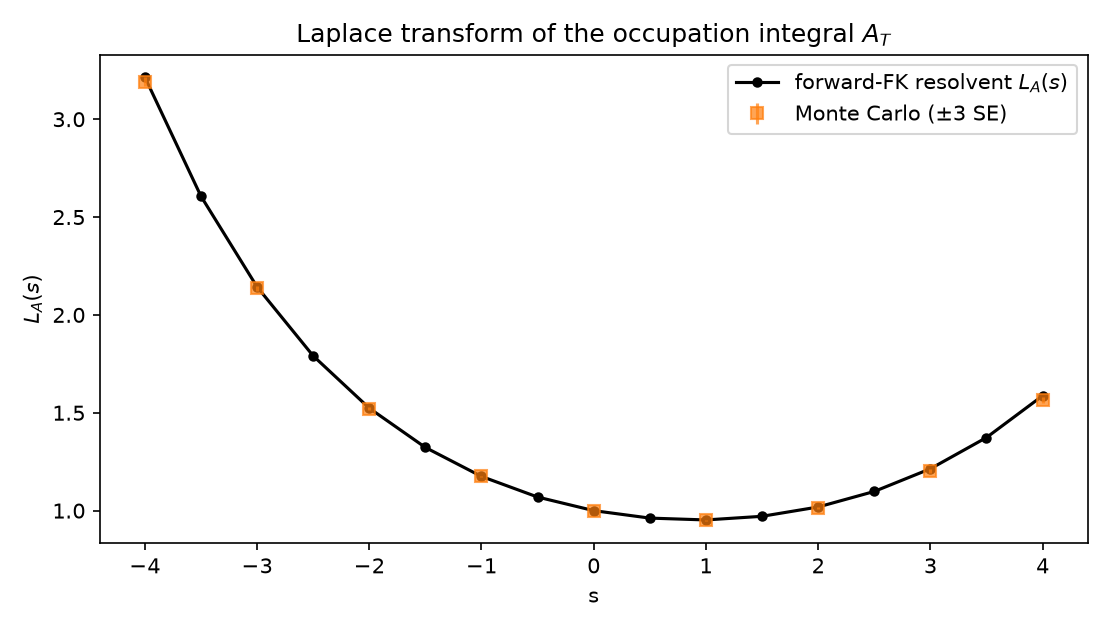
\includegraphics[keepaspectratio]{figures/phase8_mgf.png}}

}

\caption{\label{fig-mgf}Laplace transform \(L_A(s)\): forward-FK
resolvent vs exact-skeleton Monte Carlo (\(\pm3\) SE).}

\end{figure}%

\section{Deterministic pricing}\label{sec-pricing}

\subsection{Route 1: resolvent + COS}\label{route-1-resolvent-cos}

With truncation band \([a,b]=z_0\pm\kappa\sqrt{\beta T+|\alpha|T}\) and
modes \(\theta_k=k\pi/(b-a)\), the payoff coefficients of the call are
derived for \textbf{arbitrary strike position relative to the band}:

\[
G_k=\int_a^b(z-K)^+\cos(\theta_k(z-a))\,dz=
\begin{cases}
\dfrac{(-1)^k-\cos(\theta_k(K-a))}{\theta_k^2}, & K\in[a,b],\\[2ex]
\dfrac{(-1)^k-1}{\theta_k^2},\quad G_0=\dfrac{(b-K)^2-(a-K)^2}{2}, & K<a,
\end{cases}
\]

with the standard half-weight convention on \(k=0\). Strikes above the
band raise a configuration error rather than returning garbage.

\subsection{Route 2: clock-density
quadrature}\label{route-2-clock-density-quadrature}

\[
V=e^{-rT}\int Bachelier\big(z_0,\ \beta T+\alpha a,\ K\big)\,
p_{A_T}(a)\,da,
\]

with \(p_{A_T}\) the Milestone-4 Fourier density built from oscillating
frequencies only (\(|\phi_A(\xi)|\le1\)). This route avoids the
exponential tilting that makes large-\textbar{}\(s|\) resolvent
evaluations delicate, and is the robust default at extreme moneyness.

Cross-validation: routes agree to \(<2\cdot10^{-4}\); COS converges
spectrally in mode count (64→128 modes differ by \(10^{-5}\)); put--call
parity holds to \(10^{-8}\); the deterministic-clock limit reproduces
closed-form Bachelier to \(10^{-6}\). Against conditional-Gaussian Monte
Carlo (200k paths), all strikes 88--112 sit within \textasciitilde1 SE
((\textbf{tab-mc?}), Figure~\ref{fig-cosmc}).

\begin{longtable}[]{@{}lll@{}}
\caption{Spread calls under stochastic correlation: COS vs Monte Carlo.
\{\#tab-mc\}}\tabularnewline
\toprule\noalign{}
K & COS & MC (SE) \\
\midrule\noalign{}
\endfirsthead
\toprule\noalign{}
K & COS & MC (SE) \\
\midrule\noalign{}
\endhead
\bottomrule\noalign{}
\endlastfoot
88 & 11.414795 & 11.413487 (0.0059) \\
92 & 7.612942 & 7.611496 (0.0059) \\
96 & 3.898779 & 3.896773 (0.0055) \\
100 & 1.038546 & 1.037599 (0.0035) \\
104 & 0.093861 & 0.093752 (0.0010) \\
108 & 0.003107 & 0.002963 (0.00016) \\
\end{longtable}

\begin{figure}[tbp]

\centering{

\pandocbounded{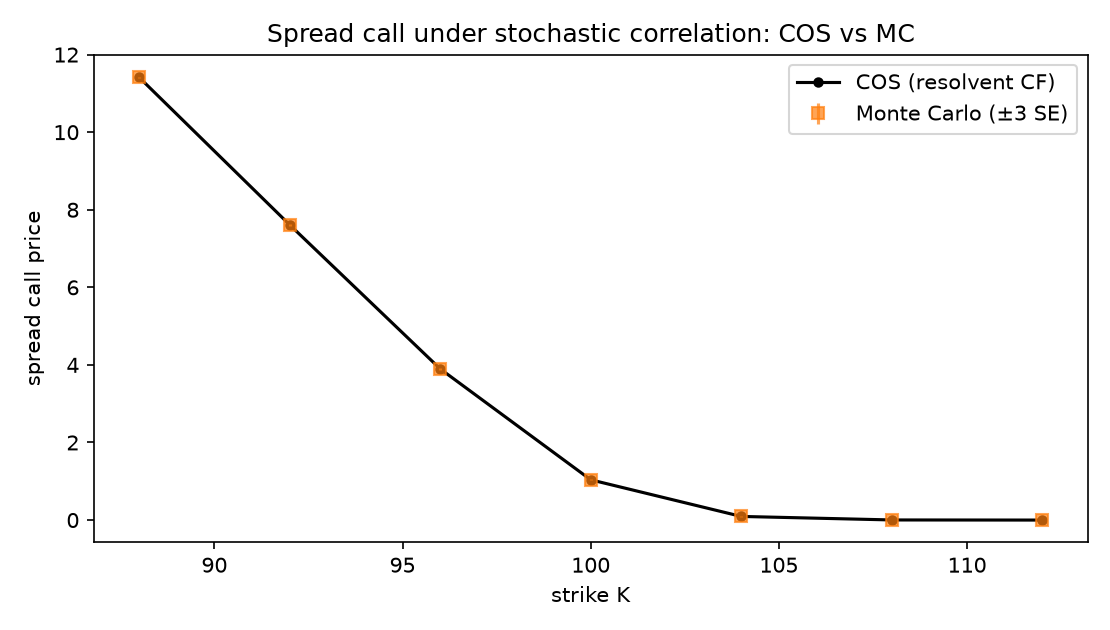
\includegraphics[keepaspectratio]{figures/phase8_cos_vs_mc.png}}

}

\caption{\label{fig-cosmc}COS prices vs Monte Carlo across strikes.}

\end{figure}%

\section{Semi-analytic Greeks}\label{sec-greeks}

With \(g(v)\) the undiscounted Bachelier call in variance \(v\),
\(d=(z_0-K)/\sqrt v\):

\[
\Delta=E[\Phi(d)],\qquad
\Gamma=E\!\left[\frac{\varphi(d)}{\sqrt v}\right],\qquad
\text{vega}_{\sigma_i}=E\!\left[\frac{\varphi(d)}{2\sqrt v}\,
\frac{\partial v}{\partial\sigma_i}\right],
\]

with
\(\partial v/\partial\sigma_1=2\alpha_1^2\sigma_1T+2\alpha_1\alpha_2
\sigma_2 A_T\) and symmetrically for \(\sigma_2\) --- all expectations
against the exact clock density. Finite-difference checks agree to
\(\le10^{-4}\) (unit suite); notebook tables agree at six decimals.

\section{Implied-correlation smiles}\label{sec-smiles}

Inverting constant-correlation Bachelier quotes against the stochastic-
correlation price produces the model's falsifiable signature
(Figure~\ref{fig-smiles}):

\begin{enumerate}
\def\labelenumi{\arabic{enumi}.}
\tightlist
\item
  both spread and basket smiles are \textbf{exactly symmetric} in
  moneyness (linear slope zero to machine precision) --- a consequence
  of the variance-mixture structure with no drift in \(Z\);
\item
  curvatures are \textbf{opposite}: spread \(-2.385\times10^{-3}\),
  basket \(+1.770\times10^{-3}\). Mechanism: variance mixtures fatten
  tails; higher wing variance maps to \emph{lower} implied correlation
  for spreads (price decreasing in \(\rho\)) and \emph{higher} for
  baskets;
\item
  ATM implied correlations recover \(E[A_T]=0.1345\) exactly --- a
  direct, assumption-light read-out of the occupation mean.
\end{enumerate}

This extends the sign corollary of the companion paper from barrier
prices to full smile geometry.

\begin{figure}[tbp]

\centering{

\pandocbounded{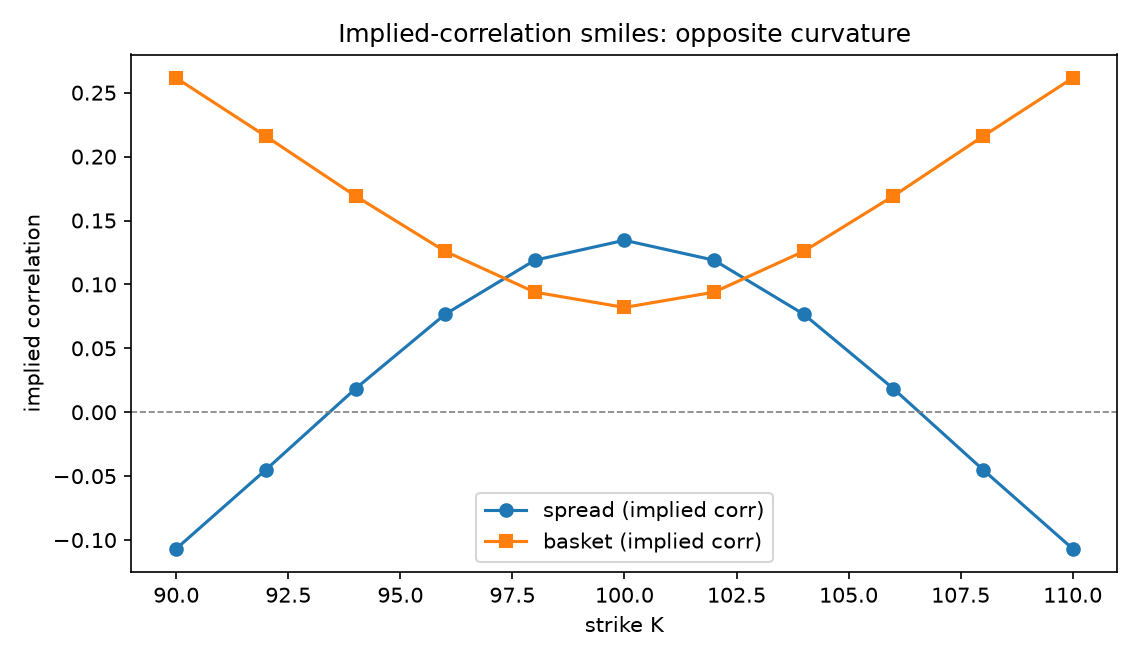
\includegraphics[keepaspectratio]{figures/phase8_implied_corr_smiles.png}}

}

\caption{\label{fig-smiles}Implied-correlation smiles: opposite
curvature for spreads and baskets.}

\end{figure}%

\section{Related literature}\label{sec-related}

The COS method is due to Fang and Oosterlee (2008); multidimensional
extensions (Ruijter and Oosterlee 2012) and their tensor-compressed
successors ({Galetzka et al.} 2026) require joint characteristic
functions and target Lévy/affine model classes without stochastic
correlation. Spread-option formulas in the lognormal/Lévy world
(Caldana--Fusai lineage) likewise assume fixed dependence. On the model
side, the audited stochastic-correlation literature (Teng et al. 2016)
offers conditional Monte Carlo only. Our contribution --- reducing the
dependence uncertainty to a bounded scalar occupation integral whose
Laplace transform is globally defined --- has no audited counterpart.

\section{Conclusion}\label{sec-conclusion}

Boundedness is not merely a mathematical convenience: it is what makes
the dependence uncertainty \emph{transformable}. One sparse PDE solve
per mode yields European spread/basket prices, Greeks, and smile
geometry at Monte Carlo accuracy, deterministically.

\section{Reproducibility}\label{sec-repro}

Environment: conda \texttt{phase3-paper} (Python 3.12.13, numpy 2.5.1,
scipy 1.18.0). Notebook \texttt{notebooks/phase8\_cos\_vanillas.ipynb}
(\textasciitilde173 s, seed 20260821); module \texttt{phase8\_cos.py};
tests \texttt{tests/test\_phase8\_cos.py} (14/14).

\protect\phantomsection\label{refs}
\begin{CSLReferences}{1}{1}
\bibitem[\citeproctext]{ref-fang2008}
Fang, Fang, and Kees Oosterlee. 2008. {``A Novel Pricing Method for
European Options Based on Fourier-Cosine Series Expansions.''}
\emph{SIAM Journal on Scientific Computing} 31 (2): 826--48.

\bibitem[\citeproctext]{ref-cosTT2026}
{Galetzka, Michiel et al.} 2026. \emph{COS-TT-CHF: Tensor Train Cosine
Method for Multivariate Option Pricing with Characteristic Functions}.

\bibitem[\citeproctext]{ref-ruijter2012}
Ruijter, Marjon, and Kees Oosterlee. 2012. {``Two-Dimensional Fourier
Cos-Series Expansion Method for Numerical Pricing of Contingent
Claims.''} \emph{SIAM Journal on Scientific Computing} 34 (5): B642--71.

\bibitem[\citeproctext]{ref-teng2016}
Teng, Long, Matthias Ehrhardt, and Michael Günther. 2016. {``Modelling
Stochastic Correlation.''} \emph{Journal of Mathematics in Industry} 6
(1): 1--18. \url{https://doi.org/10.1186/s13362-016-0018-4}.

\end{CSLReferences}




\end{document}
